\chapter{Задачи вещественной оптимизации}

\section {Функция Ackley}

\subsection {Описание функции}

\begin{tabularwide}
\textbf{Идентификатор:} & MHL\_TestFuction\_Ackley. \\
\textbf{Наименование:} & Функция Ackley. \\
\textbf{Тип:} & Задача вещественной оптимизации. \\
\end{tabularwide}

\begin{tabularwide}
\textbf{Идентификатор:} & MHL\_TestFuction\_Ackley. \\
\textbf{Наименование:} & Функция Ackley. \\
\textbf{Тип:} & Задача вещественной оптимизации. \\
\end{tabularwide}

\textbf{Формула} (целевая функция):
\begin{equation}
\label{TestFunctions:eq:MHL_TestFuction_Ackley}
f\left( \bar{x}\right) = 20 + e - 20e^{-0.2\sqrt{\frac{1}{n}\sum_{i=1}^{n}\bar{x}_i^2}}-e^{\frac{1}{n}\sqrt{\sum_{i=1}^{n}cos\left( 2\pi\cdot\bar{x}_i\right) }}, \text{ где}
\end{equation}
\indent $\bar{x}\in X$, $\bar{x}_j\in \left[ Left_j; Right_j\right] $, $Left_j=-5$, $Right_j=5$, $j=\overline{1,n}$.

\begin{tabularwide}
\textbf{Обозначение:} &\specialcell{$\bar{x}$ --- вещественный вектор;\\$n$ --- размерность вещественного вектора.}  \\
\textbf{Решаемая задача оптимизации:} & $\bar{x}_{min}= \arg \min_{\bar{x}\in X} f\left( \bar{x}\right)$.   \\
\textbf{Точка минимума:} & $\bar{x}_{min}={\left( 0,0,\ldots,0\right)}^\mathrm{T} $, то есть $\left(\bar{x}_{min} \right)_j=0$ ($j=\overline{1,n}$).    \\
\textbf{Минимум функции:} & $f\left(\bar{x}_{min} \right) =0$.   \\
\textbf{График:} & Рисунок \ref{TestFunctions:img:MHL_TestFuction_Ackleye} нас \pageref{TestFunctions:img:MHL_TestFuction_Ackleye} стр.   \\
\end{tabularwide}

\textbf{}
\begin{figure} [h] 
  \center
  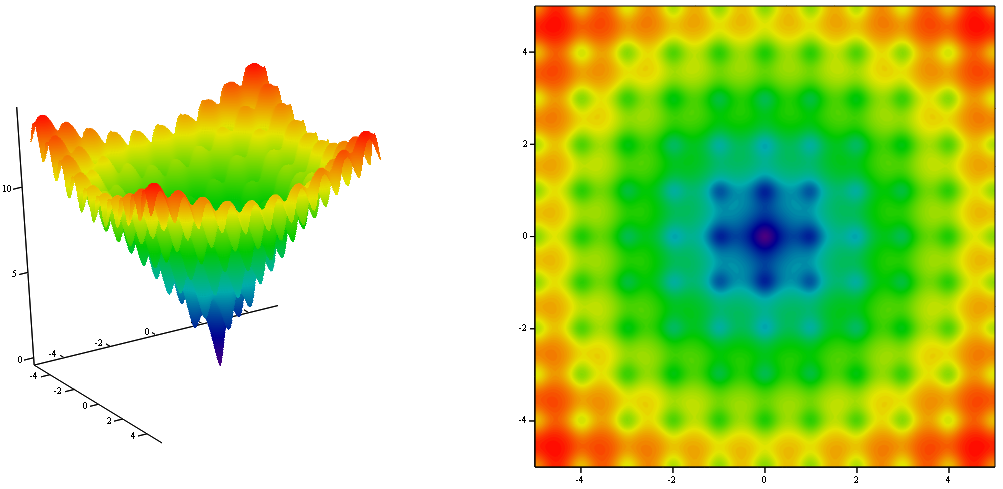
\includegraphics [scale=0.5] {MHL_TestFuction_Ackley}
  \caption{Функция Ackley} 
  \label{TestFunctions:img:MHL_TestFuction_Ackleye}  
\end{figure}

\subsection {Параметры для алгоритмов оптимизации}

\begin{tabularwide}
\textbf{Точность вычислений:} & $\varepsilon=0.025$. \\
\textbf{Число интервалов, на которые предполагается разбивать каждую компоненту вектора $\bar{x}$ в пределах своего изменения} (для алгоритмов дискретной оптимизации) : & $NumberOfParts_j=4095$ ($j=\overline{1,n}$). \\
\end{tabularwide}

\textbf{Замечание:}  $NumberOfParts_j$ выбирается как минимальное число, удовлетворяющее соотношению:
\begin{equation*}
NumberOfParts_j=2^{\left( k_2\right)_j }-1\geq\dfrac{10\left( Right_j-Left_j\right) }{\varepsilon},\text{где } \left( k_2\right)_j \in \mathbb{N}, \left( j=\overline{1,n}\right).
\end{equation*}

\subsection {Основная задача и подзадачи}

\begin{tabularwide}
\textbf{Изменяемый параметр: } & $n$ --- размерность вещественного вектора. \\
\textbf{Значение в основной задаче:} & $n=2$.\\
\textbf{Подзадача №2:} & $n=3$.\\
\textbf{Подзадача №3:} & $n=4$.\\
\textbf{Подзадача №4:} & $n=5$.\\
\textbf{Подзадача №5:} & $n=10$.\\
\textbf{Подзадача №6:} & $n=20$.\\
\textbf{Подзадача №7:} & $n=30$.\\
\end{tabularwide}

\subsection {Нахождение ошибки оптимизации}

Пусть в результате работы алгоритма оптимизации за $N$ запусков мы нашли решения $\bar{x}_{submin}^k$ со значениями целевой функции $f\left( \bar{x}_{submin}^k\right) $ соответственно ($k=\overline{1,N}$). Используем три вида ошибок:

\textbf{Надёжность: }
\begin{equation*}
R = \dfrac{\sum_{k=1}^{N}S\left( \bar{x}_{submin}^k \right) }{N}, \text{ где}
\end{equation*}
\begin{equation*}
S\left( \bar{x}_{submin}^k \right)=\left\lbrace \begin{aligned} 1,& \text{ если } \left| \left( \bar{x}_{submin}^k \right)_j-\left( \bar{x}_{min} \right)_j\right|\leq\varepsilon, j=\overline{1,n};   \\ 0,& \text{ иначе}. \end{aligned}\right.
\end{equation*}

\textbf{Ошибка по входным параметрам:}
\begin{equation*}
E_x = \dfrac{\sum_{k=1}^{N} \left( \frac{\sqrt{\sum_{j=1}^{n}{\left( \left( \bar{x}_{submin}^k \right)_j-\left( \bar{x}_{min} \right)_j \right)}^2 }}{n} \right)  }{N}.
\end{equation*}

\textbf{Ошибка по значениям целевой функции: }
\begin{equation*}
E_f = \dfrac{\sum_{k=1}^{N} \left| f\left( \bar{x}_{submin}^k \right)-f\left( \bar{x}_{min} \right) \right|  }{N}.
\end{equation*}

\subsection {Свойства задачи}
\begin{tabularwide}
\textbf{Условной или безусловной оптимизации: } & Задача безусловной оптимизации. \\
\textbf{Одномерной или многомерной оптимизации: } & Многомерной: $ n $. \\
\textbf{Функция унимодальная или многоэкстремальная: } & Функция многоэкстремальная. \\
\textbf{Функция стохастическая или нет: } & Функция не стохастическая. \\
\textbf{Особенности: } & Нет. \\
\end{tabularwide}

\subsection {Реализация}

Реализация функции взята из библиотеки MathHarrixLibrary в разделе <<Тестовые функции для оптимизации>>, которую можно найти по адресу \href{https://github.com/Harrix/MathHarrixLibrary} {https://github.com/Harrix/MathHarrixLibrary}.

\begin{lstlisting}[caption=Код функции MHL\_TestFuction\_Ackley]
double MHL_TestFuction_Ackley(double *x, int VMHL_N)
{
/*
Функция многих переменных: Ackley.
Тестовая функция вещественной оптимизации.
Входные параметры:
 x - указатель на исходный массив;
 VMHL_N - размер массива x.
Возвращаемое значение:
 Значение тестовой функции в точке x.
*/
double VMHL_Result;
double f1,f2=0;
f1=exp(-0.2*sqrt(TMHL_SumSquareVector(x,VMHL_N)/double(VMHL_N)));
for (int i=0;i<VMHL_N;i++) f2=f2+cos(2.*MHL_PI*x[i]);
f2=exp(f2/double(VMHL_N));
VMHL_Result=20.+exp(1)-20.*f1-f2;
return VMHL_Result;
}
\end{lstlisting}

\subsection {Ссылки}

Данная функция приводится в следующих источниках:

\begin{enumerate}
\item \cite[стр. 5]{web:1207.4318} ---  \href{http://arxiv.org/pdf/1207.4318v1.pdf}{Empirical review of standard benchmark functions using evolutionary global optimization}.
\item \cite{web:www.cs.unm.edu:AckleysFunction} ---  \href{http://www.cs.unm.edu/~neal.holts/dga/benchmarkFunction/ackley.html}{Ackley's Function}.
\end{enumerate}

\clearpage